\section{Cryptocurrencies correlation}
\label{sec:crypto_corr}

Blockchain was specifically designed to work with cryptocurrencies. In fact,
transactions work very well for transfering money from a user to another, while
every block works like an archive of them, allowing everyone to browse
the chain history and check every money movement.

Miners get a reward for every transaction and for every block processed,
usually in the current cryptocurrency. This kind of reward mitigates attackers
to try to modify the blockchain to have back their funds.

Any user holds at least one \textbf{wallet}, that has a specific address. An
address is a random-generated token 26-35 alphanumeric characters long. Users
can have more than one wallet, and creating a new one does not require any
authentication.

Money can be sent to non-existing wallets. These money transfers are saved in
the chain and if someone creates a wallet with the exact token it will be able
to redeem them.

\subsection{Privacy during transactions}

With cryptocurrencies sometimes it is important to keep some kind of privacy
during a transaction. There are different countries in the world where
fundamental liberties do not exists, mass surveillance is a threat for
people and even a simple movement of money online can constitute a problem.
Due the fact that every transaction is broadcast to the network there is no
privacy about the its content. Everyone can see how much is sent to
other addresses. Many websites provide functionalities \footnote{For example,
\url{https://blockexplorer.com/} enable users to search in the Bitcoin
Blockchain.} that allow anyone to easily search data in a working Blockchain
implementation.

Wallets are usually defined as ``pseudo anonymous'', meaning that until the
user does not link any personal information with that address she is anonymous.
This form of anonymity is not strong because it is quite easy for an attacker to
track the transaction history of a user and to infer information about her of
her habits.
There are different studies \cite{guadamuz15} that point out how it is
relatively easy for an attacker to discover user information thanks
to payments on online shops. An user could buy some goods from an online store
with a cryptocurrency, where she is registered with a username and password,
linking \textit{de facto} her identity with her wallet.
The IP address also plays a role~\cite{koshy14} and with statistical analysis
is possible to link an IP address with a wallet, making it easier to track user
identity.
Fortunately, there are online services that make IP and address tracking more
difficult: these services are known as \textbf{mixers} and are usually websites
that send amount of money from an address to the other, ensuring that during the
transfer additional money movement is done in different ways, making more
difficult for an attacker to track the original payer. This can enhance the
privacy and mitigate the problem, making more difficult to rebuild history of
transactions for a single user, at the cost of more transfer fees. Using mixers
means that some form of thrust is placed in the service owner, than could be an
attacker itself eavesdropping users that are searching for more privacy.

\subsection{Account and Keys management}

User and account concepts do not exist in the Blockchain implementation per-se.
Therefore there is not any real account management, and no password
authentication. In its financial implementations, recovering a lost wallet is
usually almost impossible, because if the asymmetric keys are lost there is no
way to reclaim the transactions, hence to reclaim the money. This Blockchain
characteristic lead to money being locked-in forever into lost accounts in
cryptocurrencies.
It is important to note, by the way, that Blockchain implementations that differ
from Nakamoto's original idea could have a different account management, as for
example in\cite{azaria16} where the access to the blockchain is regulated via
prior authentication, or in\cite{zhou16} where the authors added an
authentication layer to better manage Bitcoin accounts.

\begin{figure}[ht]
 \centering
 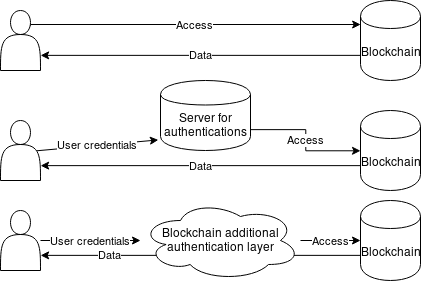
\includegraphics[scale=0.5]{authenticationMethods}
 \label{img:authMethods}
 \caption[Different ways to access a Blockchain database]{Different ways to
access a Blockchain database:
 \begin{enumerate*}[label=\arabic*)]
  \item without any extra authentication,
  \item via a separated server that manages user authentication,
  \item adding another verification layer.
 \end{enumerate*}}
\end{figure}

This highlights the importance for a user to keep a backup of her keys. Wallet
keys can be stored in different ways.

\paragraph{Digital Copy} One could make a simple digital copy of the key on a
digital storage (for example an USB key), but this would lead to expose the
keys to several vulnerabilities: first of all, the keys could be stolen or lost.
Even having the keys in a physical media without any protection system is
dangerous: as explained in\cite{eskandari15}, an attacker could spread a
malware able to send to her copies of users' private keys. Encrypting the keys
would work only to mitigate theft attacks, but a malware could always be
shipped with a keylogger, nullifying this protection.

Coping the key online on some storage service or cloud will not enhance its
security either, because there is the possibility that the service provider
reads the user data, or that the service suffers an attack and leaks its
content.

A possible solution to effectively protect the keys with these backups is
requiring a multi-factor authentication system to decrypt them, enhancing the
security but with a usability degradation.

\paragraph{Physical Copy} There is the possibility for currencies like Bitcoin
to print the wallet address and its private key into a piece of paper. This
system though is not safe as it seems, because they are exposed, like the
media storage, to the possibility of being stolen or the possibility to be lost.
Another threat is that the key could be easily seen and
copied~\cite{eskandari15}.
